\documentclass[10pt,a4paper,twoside]{article}
\usepackage[a4paper,top=20mm,bottom=20mm,outer=5cm]{geometry}
\usepackage[utf8]{inputenc}
\usepackage[english]{babel}
\usepackage{graphicx}
\usepackage{hyperref}
\usepackage{amsmath}
\usepackage{cleveref}
\usepackage{natbib}
\bibliographystyle{abbrvnat}
\setcitestyle{authoryear}

\title{Project Machine Learning\\--- Milestone 1 ---} 

%%%%%%%%%%%%%%%%%%%%%%%%%%%%%%%%%%%%%%%
%                                     %
%   EVERYTHING BELOW CAN BE CHANGED   %
%                                     %
%%%%%%%%%%%%%%%%%%%%%%%%%%%%%%%%%%%%%%%

\author{Konstantin Ausborn, Timon Palm, Marco Rosinus Serrano}
\date{\today}

\begin{document}
\maketitle

\section{Introduction}


\section{Vector-Quantized variational Autoencoder (VQ-VAE)}
\label{sec:vqvae}

% explain handling of different image sizes

\section{Dataset overview}
    Vectore-quantised variational autoencoders (VQ-VAE) are applicable to different modalities, like image, video or audio generation. 
    By virtue of comparison with its predecessors (Autoencoder, VAE) and the paper itself, we will first focus on image generation only.

    The performance of the VQ-VAE was showcased on three different image datasets: \textit{ImageNet}, \textit{CIFAR-10} and Video frames from \textit{DeepMind Lab}.

    In this project, we will train and test our implementation on ImageNet as well as CIFAR-10, which makes our results comparable to the original paper but also to other generative architures.

    Image generation is an unsupervised learning task and therefore does not require labeled data. Potentially, any kind of image data could be used for training and testing. However, the quality of the generated images is highly dependent on the quality and diversity of the training data.

    ImageNet and CIFAR-10 are among the most common image datasets. They are both created for image classification tasks, but we can also leverege their capacity by simply dropping their labels. Table \ref{tab:datasets} gives an overview of the datasets.
    
    \subsection{ImageNet}
    ImageNet is a widely used image datasets in the field of machine learning, primarily for the task of classification and detection.
    The full dataset consists of 14.197.122 hand-labeled photographs collected from flickr and other search engines \cite{ILSVRC15}. The images are distributed over 21841 \textit{synonym sets} from the \textit{WordNet} \cite{wordnet} hierarchy.

    When talking about ImageNet, most authors refer to the \textit{ImageNet Large Scale Visual Recognition Challenge 2012} (ILSVRC) dataset \cite{ILSVRC15}, which is a subset of the full dataset. It contains 1.281.167 unique labeled training images and 100.000 labeled test images, which are distributed over 1000 classes. ILSVRC is an image classification/recognition challenge. It therefore additionally contains 50.000 validation images without labels as part of the benchmark. There are neither missing values nor duplicates in the dataset and every image belongs to exactly one class.

    In the following, we will refer to the ILSVRC 2012 dataset as ImageNet if not stated otherwise.

    As the number of samples and classes hint, the data can not be balanced. In fact, the number of images per class varies from 732 to 1300 images in the training set (\ref{fig:imnet_dist}). Among the classes with the lowest number of images are \textit{"black-and-tan coonhound"}, \textit{"otterhound"} and \textit{"English foxhound"} with 732, 738 and 754 number of samples, respectively. 

    \begin{figure}
        \centering
        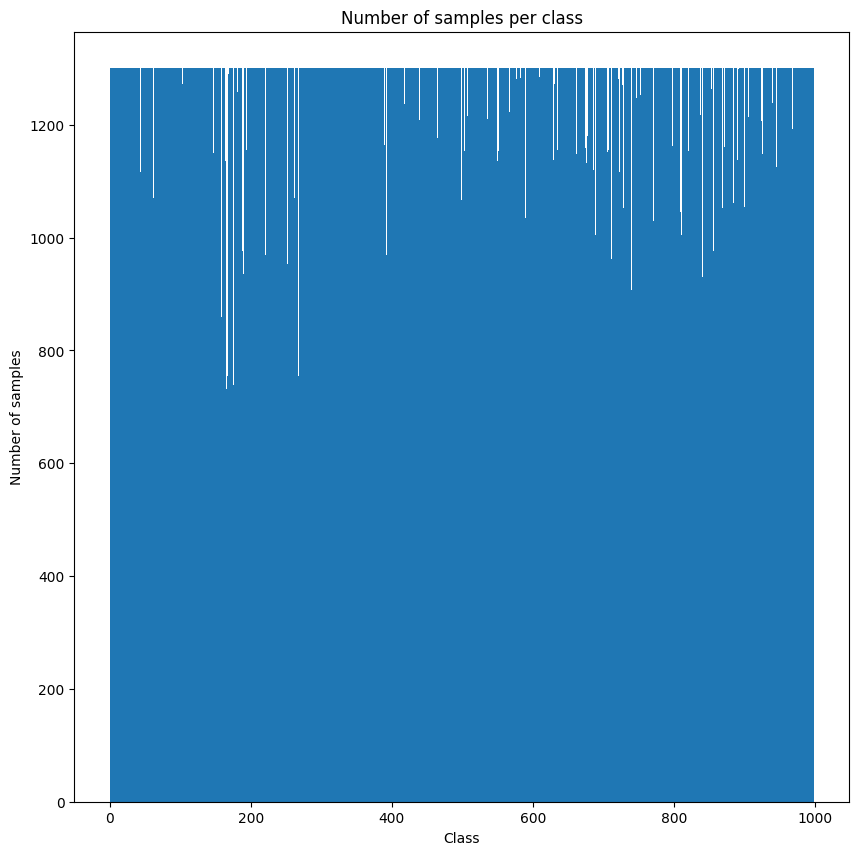
\includegraphics[width=\textwidth]{../../sample_images/imagenet_dist.png}
        \caption{Distribution of images per class in the ImageNet dataset}
        \label{fig:imnet_dist}
    \end{figure}

    Images in the ILSVRC dataset have a wide range of resolutions, from 75x56 pixels to 4288x2848 pixels and an average resolution of 469x387 pixels. While technically a VQ-VAE can handle different images sizes (see section \ref{sec:vqvae}), we will preprocess all images to a fixed size for training and testing. 

    \subsubsection{Preprocessing}
    For training and testing, we will resize all images to 128x128 pixels, as it was also done in the paper. By virtue of the VQ-VAE architecture, this implies a latent space of 32x32x1 pixel.

    There are different ways to resize the images, like cropping, padding or resizing. We will use random cropping to extract a square image and resize it to 128x128 pixels. This way, we can also handle smaller images without disturbing them or augmenting them with padding.


    Although \textit{data whitening/standardization} is not as important for Convoluational Neural Networks (CNNs), which VQ-VAE ultimately is build of, it is still a suggested procedure for ImageNet data. ImageNet whitening was also done for training the common
    \textit{Resnet} architecture \cite{resnet} on ImageNet. Furthermore, it is in the standard tensorflow and pytorch preprocessing pipeline for ImageNet class.

    Example images from ImageNet dataset are depicted in figure \ref{fig:imnet_example} (before whitening) and \ref{fig:imnet_example_normalized} (after whitening).

    \subsection{CIFAR-10}
    CIFAR-10 \cite{cifar10} is another popular image classification dataset, as well as the larger version CIFAR-100. CIFAR-10 consists of 60.000 32x32 pixel images, which are distributed over 10 classes. The dataset is split into 50.000 training images and 10.000 test images. The classes are mutually exclusive, which means that each image belongs to exactly one class. The classes are: \textit{airplane, automobile, bird, cat, deer, dog, frog, horse, ship, truck}

    The train set contains exactly 5000 images per class, while the test set contains 1000 images per class.

    There is no further preprocessing necessary for CIFAR-10, as the images are already 32x32 pixels and have a fixed size.

    \begin{table}[]
        \begin{tabular}{lllll}
        Dataset & \# train images & \# test images & \# classes & image size \\ \hline \hline
          ImageNet (ILSVRC)  & 1.281.167    &        100.000        &      1000       &    75x56px - 4288x2848px       \\
        CIFAR-10   &        50.000     &      10.000      &    10    &     32x32px       \\ \hline \hline
        \end{tabular}
        \caption{Datset overview: ImageNet and CIFAR-10}
        \label{tab:datasets}
    \end{table}

\section{Baseline method and evaluation}

\begin{itemize}
    \item basically just use negative log entropy as the factor to compare
    \item this describes the entropy of the picture generated?
    I do not have clarity here see: https://bjlkeng.io/posts/a-note-on-using-log-likelihood-for-generative-models/
    \item I need to understand PixelCNN better to continue
    \item see Shannon for theory on entropy\cite{shannon}
    \item dont use parzen windows\cite{note_on_eval}
    \item
    \item
\end{itemize}

\section{Discussion}
:-)

\bibliography{bibliography}

\section{Appendix}
\begin{figure}
    \centering
    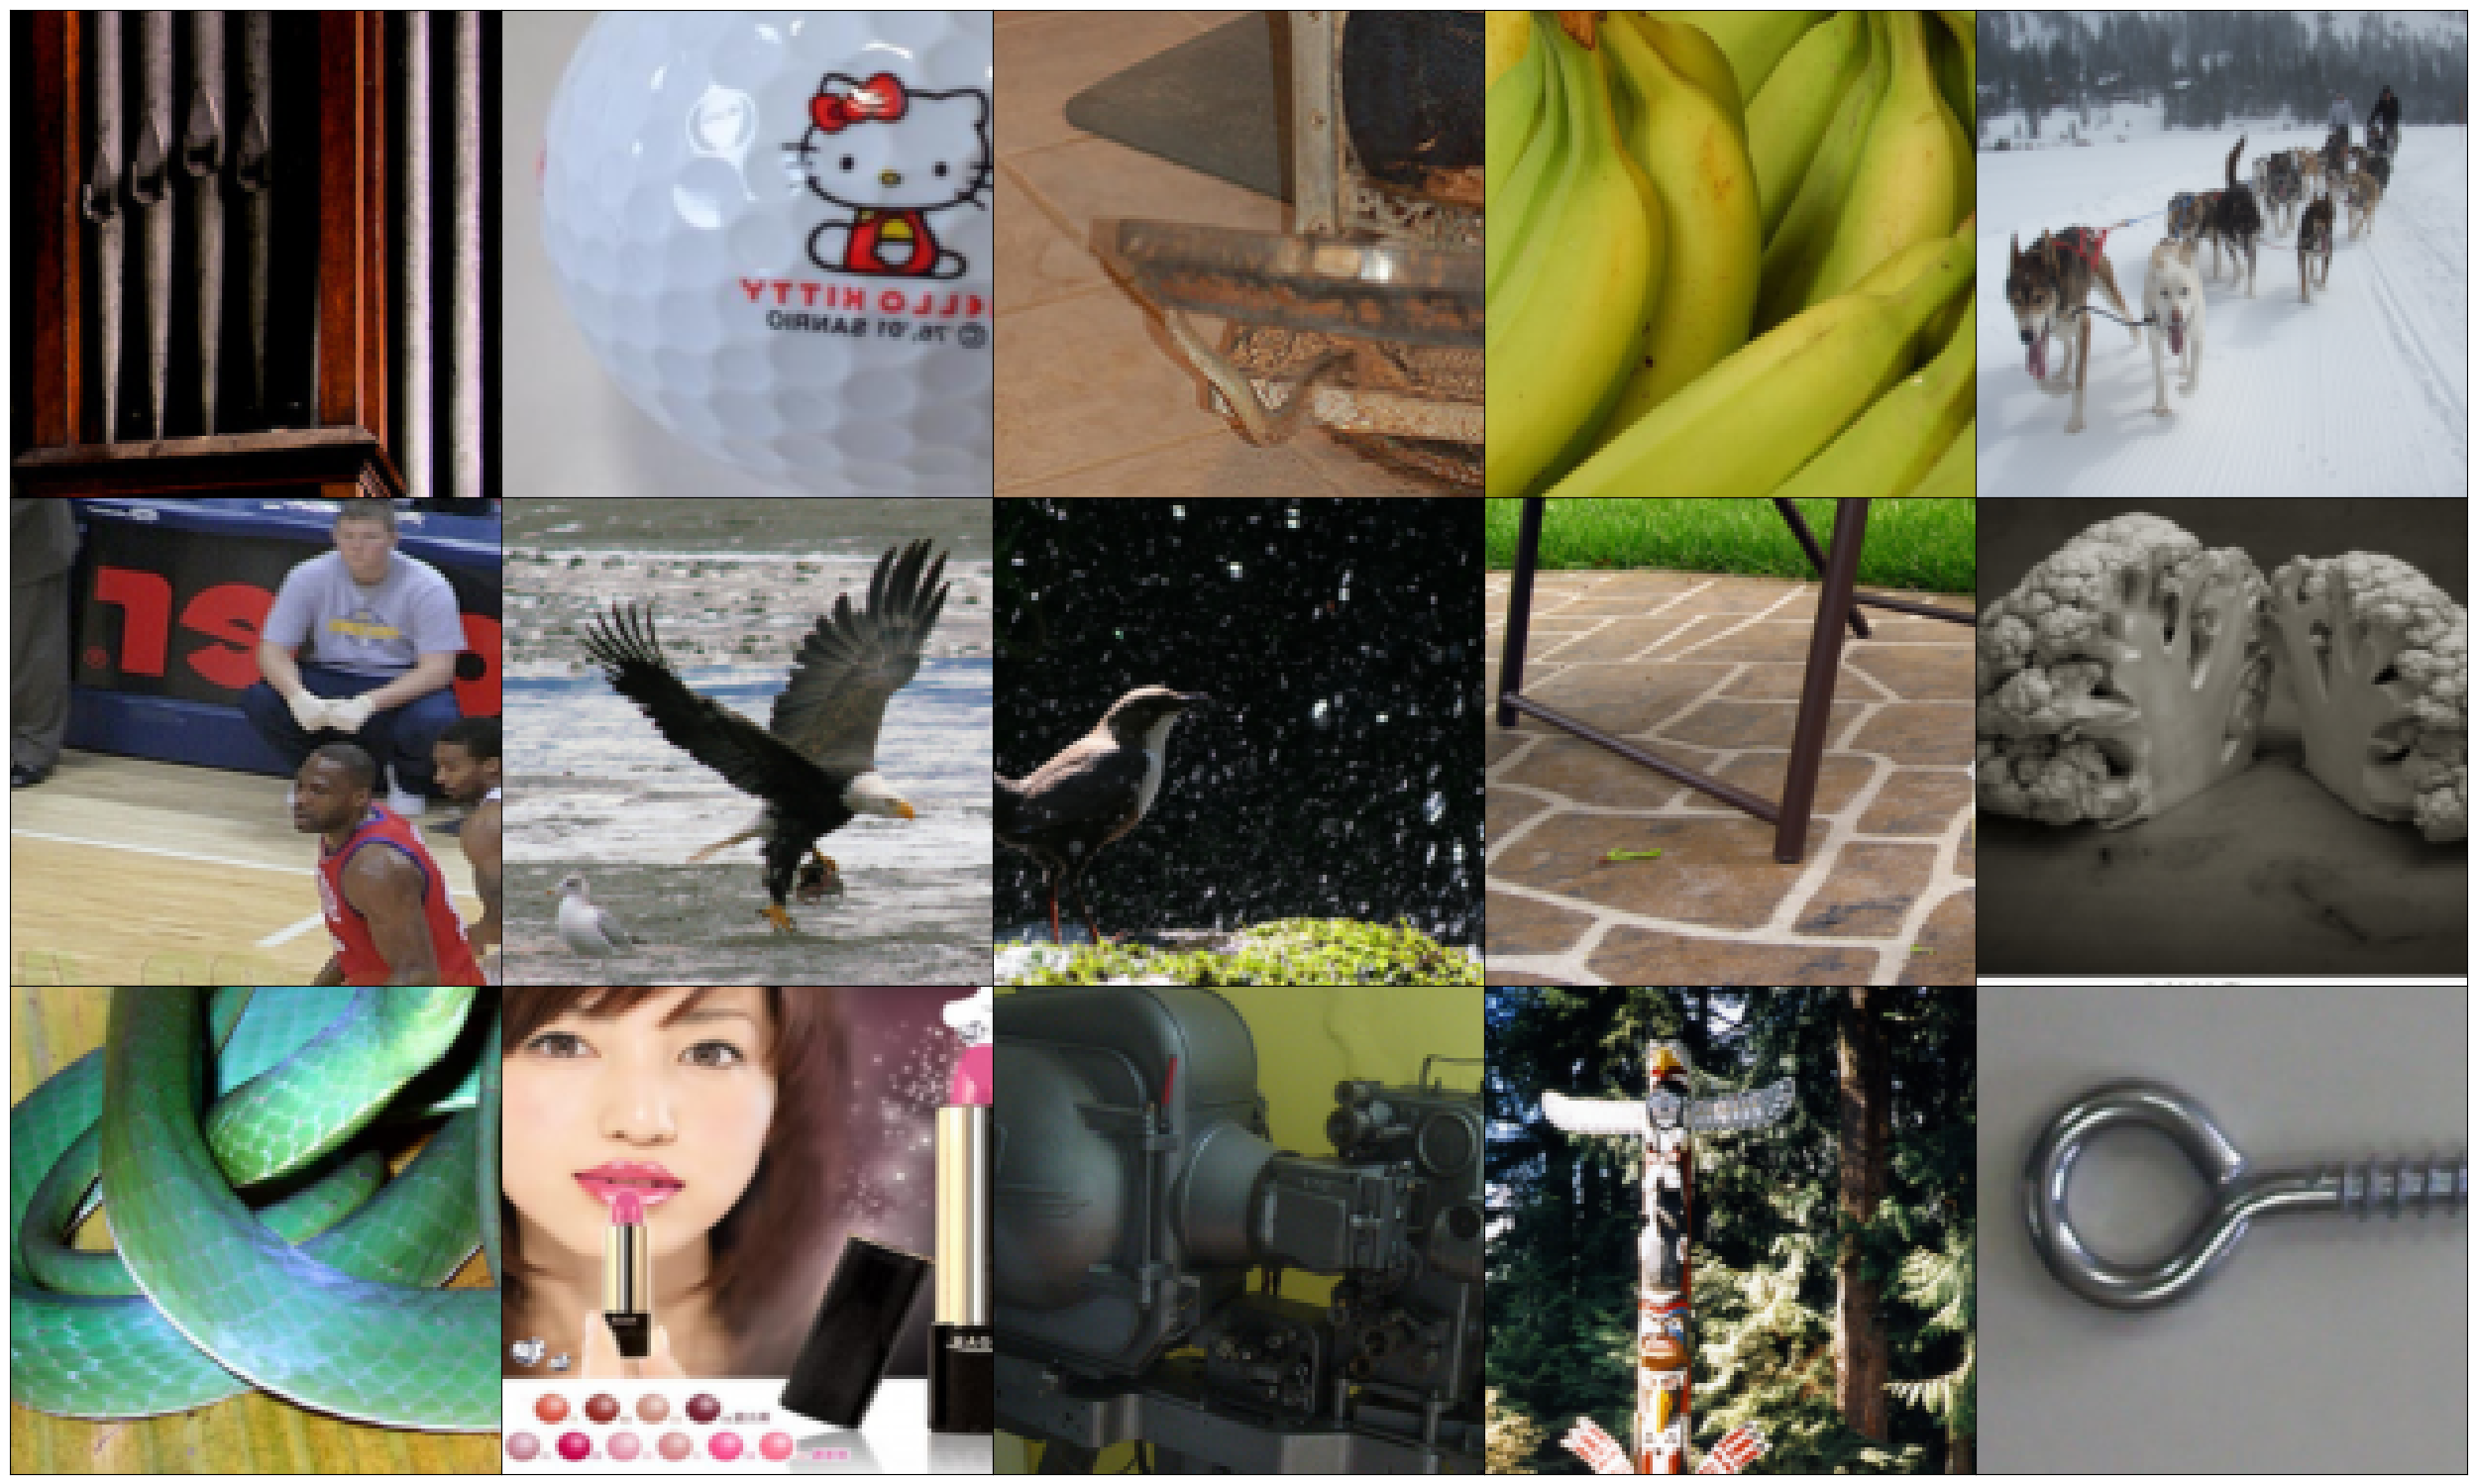
\includegraphics[width=\textwidth]{../../sample_images/imagenet_unnormalized.png}
    \caption{Example images from the ImageNet dataset randomly cropped and resized to 128x128 pixels}
    \label{fig:imnet_example}
\end{figure}
\begin{figure}
    \centering
    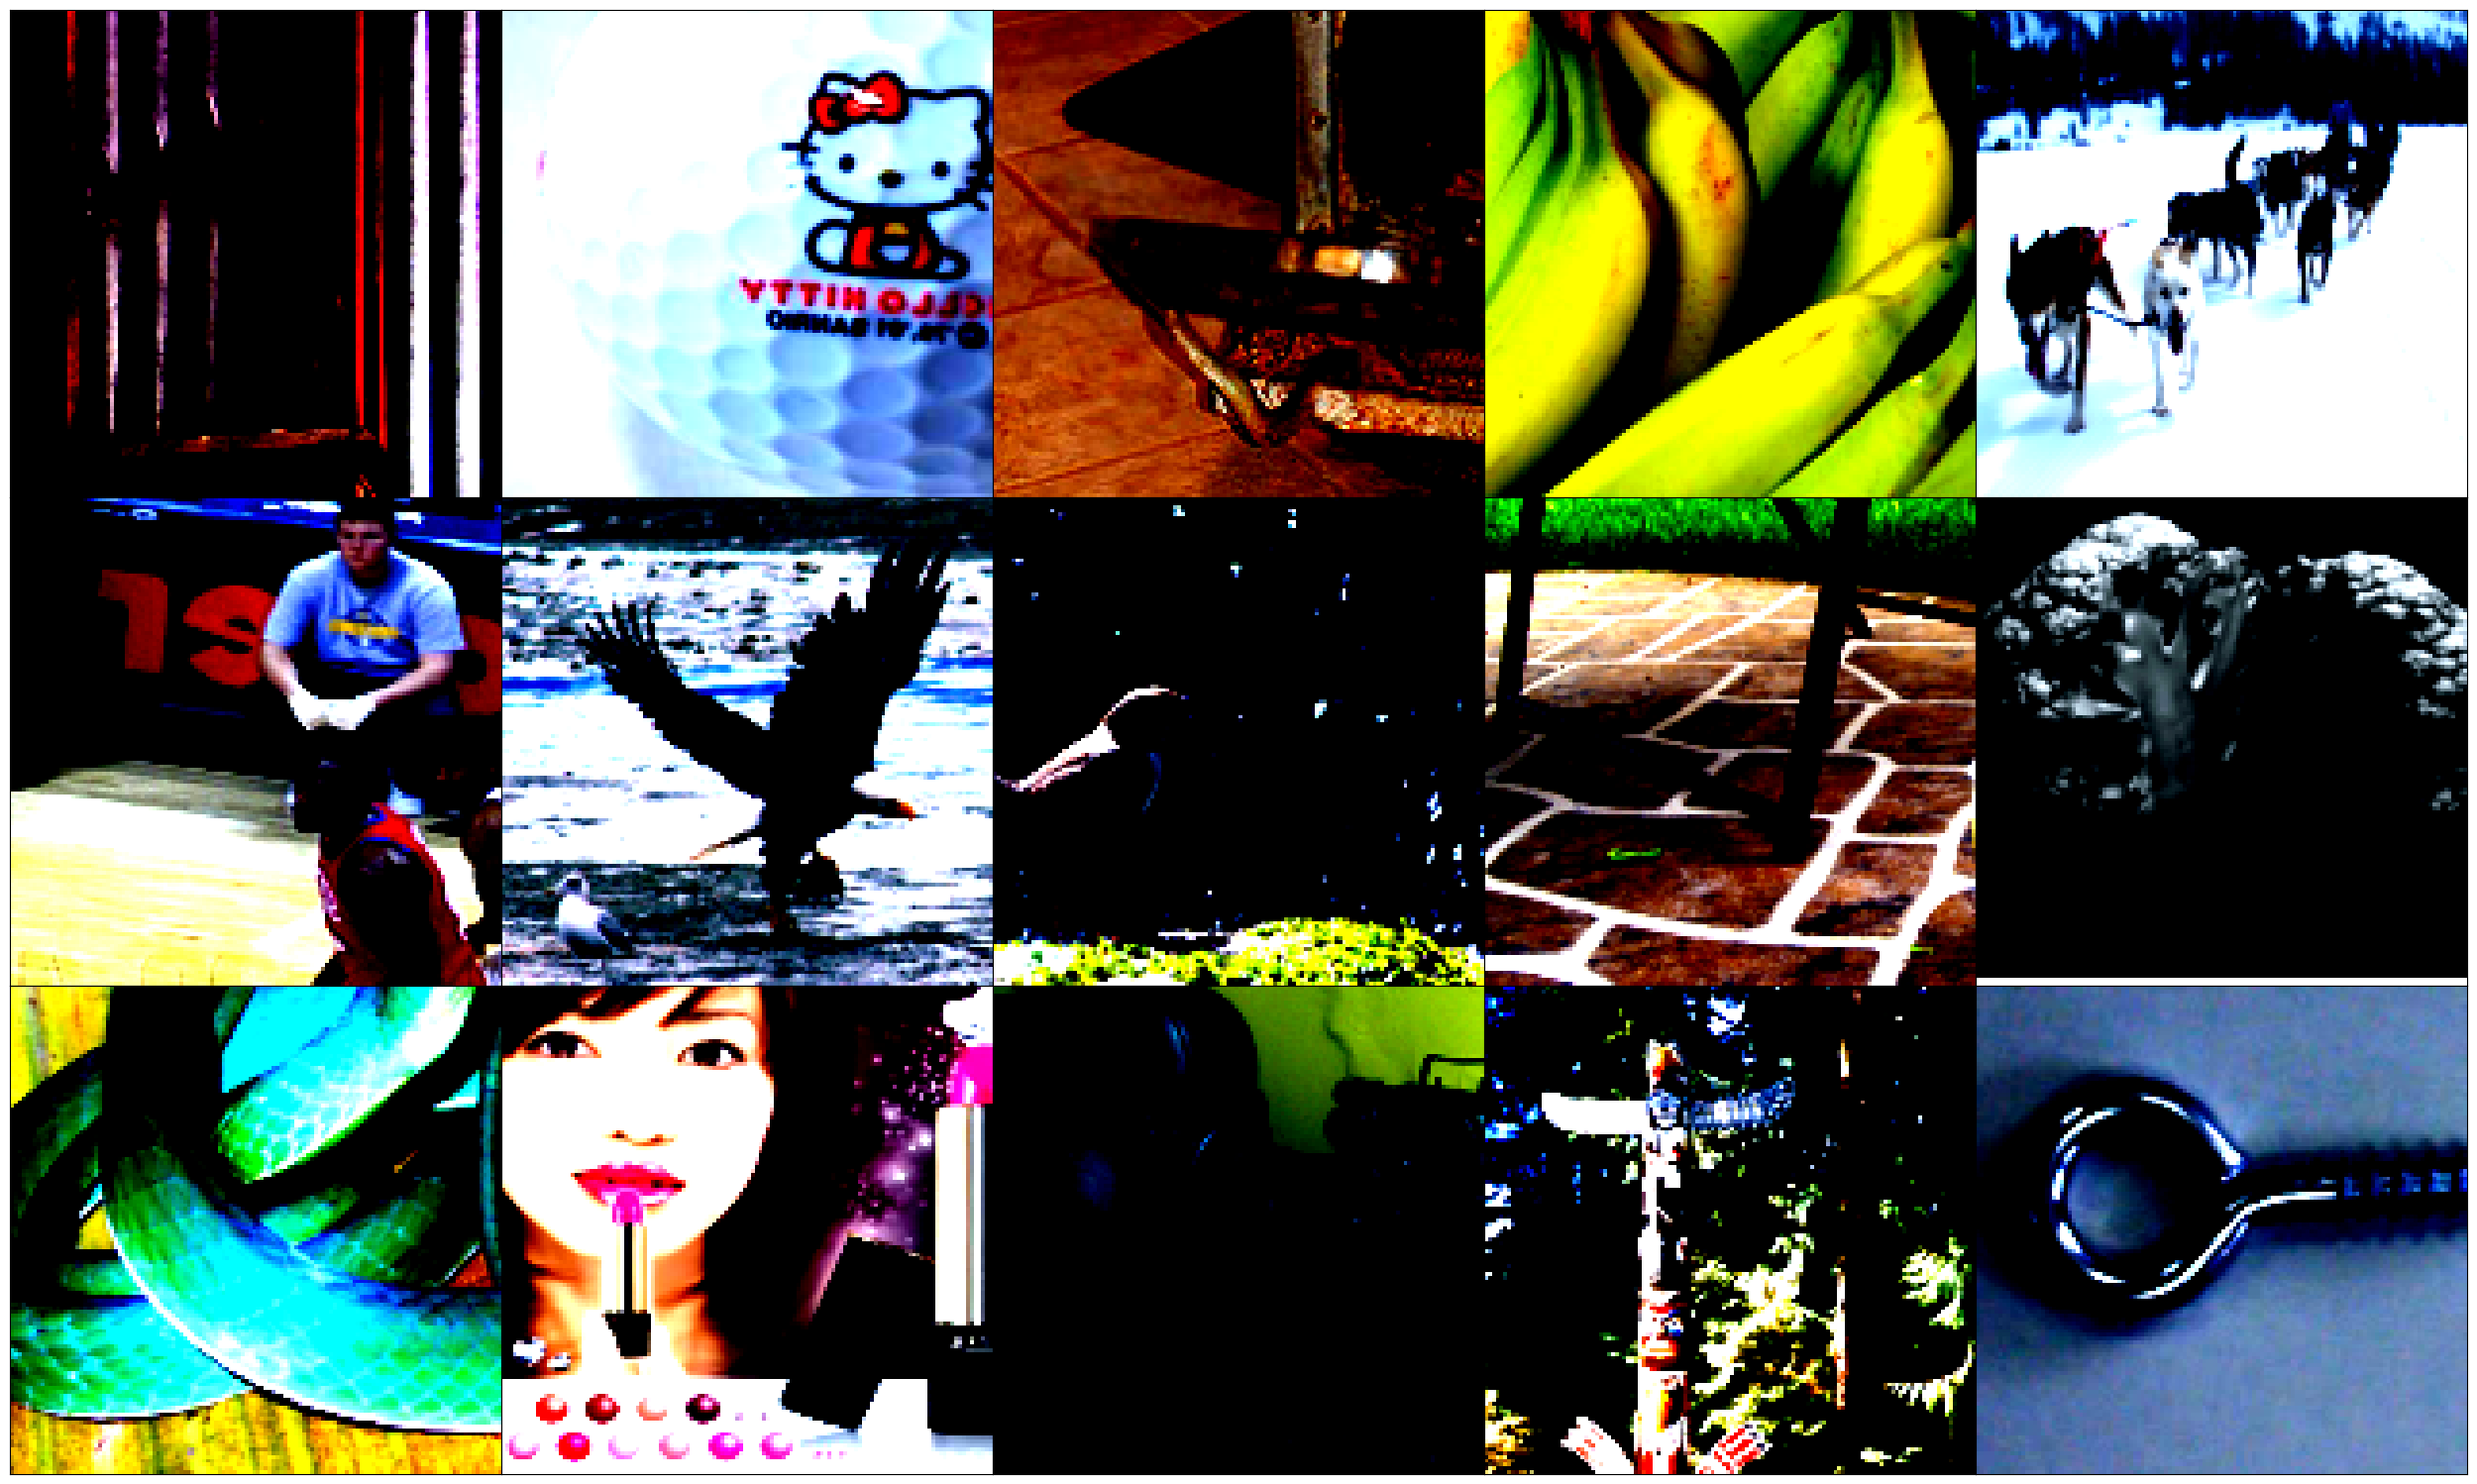
\includegraphics[width=\textwidth]{../../sample_images/imagenet_normalized.png}
    \caption{Example images from the ImageNet dataset randomly cropped and resized to 128x128 pixels and standardized}
    \label{fig:imnet_example_normalized}
\end{figure}

\end{document}
